\documentclass[11pt,a4paper]{book}
\usepackage[UTF8]{ctex} % 必须保留，用于中文支持

% --- 基础数学与核心宏包 ---
\usepackage{amsmath, amssymb, amsfonts}
\usepackage{geometry}
\usepackage{bm}
\usepackage{tcolorbox}
\usepackage{xcolor}
\usepackage{graphicx}
\usepackage{caption}
\usepackage{subcaption}
\usepackage{float}
\usepackage{multirow} % 必须要有这个，否则 \multirow 命令会报错
\usepackage{booktabs}
\usepackage{listings}
\usepackage{enumitem}
\usepackage{array}
\definecolor{codegreen}{rgb}{0,0.6,0}
\definecolor{codegray}{rgb}{0.5,0.5,0.5}
\definecolor{codepurple}{rgb}{0.58,0,0.82}
\definecolor{backcolour}{rgb}{0.95,0.95,0.92}


% 代码块样式全面升级
\lstset{
    backgroundcolor=\color{backcolour},   
    commentstyle=\color{codegreen},
    keywordstyle=\color{blue},
    numberstyle=\tiny\color{codegray},
    stringstyle=\color{orange},
    basicstyle=\ttfamily\small,
    breakatwhitespace=false,         
    breaklines=true,                 
    captionpos=b,                    
    keepspaces=true,                 
    numbers=left,                    
    numbersep=5pt,                  
    showspaces=false,                
    showstringspaces=false,
    showtabs=false,                  
    tabsize=4,
    language=R,
    frame=single,
    rulecolor=\color{black!30}
}

% --- 绘图支持 ---
\usepackage{tikz}
\usetikzlibrary{shapes, arrows, positioning} 

\usepackage[
    colorlinks=true,
    linkcolor=blue,
    unicode=true
]{hyperref}









\geometry{left=2cm, right=2cm, top=2.5cm, bottom=2.5cm}
\begin{document}

% --- 重新设计的简单封面 ---
\begin{titlepage}
    \centering
    
    \vspace*{2cm} % 稍微调高了顶部间距以平衡视觉
    
    % 顶部的两条横线
    \rule{\textwidth}{1pt}\par
    \vspace{0.2cm}
    \rule{\textwidth}{3pt}\par
    
    \vspace{1.5cm}
    
    {\Huge \bfseries R语言自学笔记 \par}
    \vspace{0.5cm}
    {\Large \itshape R \par} % 修正了 Rigid 的拼写
    
    \vspace{1cm}

    

    \vspace{1cm}
    
    \rule{\textwidth}{3pt}\par
    \vspace{0.2cm}
    \rule{\textwidth}{1pt}\par
    
    \vspace{2cm}
    \begin{center}
        
\includegraphics[width=0.4\textwidth]{Figure/R语言图标.jpg} \\ % 这里可以
        \vspace{0.5cm}
    \end{center}
    \begin{flushright}
        {\Large \textbf{魏舟} } \\
        \vspace{0.5cm}
        {\large \today}
    \end{flushright}
    
     
    \vfill
    
    {\color{gray} \footnotesize 自己捯饬R语言的笔记}

\end{titlepage}

\tableofcontents

\chapter{R语言简介}
R 语言不仅是一门编程语言，更是数据科学领域处理复杂统计逻辑的专业环境。其核心竞争力在于将严谨的数学模型与出版级的数据可视化（Data Visualization）完美融合。不同于通用编程语言，R 的设计哲学高度契合数学直觉，例如在处理标准正态分布 $N(0, 1)$ 的概率密度计算时：
\begin{equation}
f(x) = \frac{1}{\sqrt{2\pi}} e^{-\frac{x^2}{2}}
\end{equation}
开发者仅需调用 \texttt{dnorm(x)} 即可实现。



在图形生成方面，R 的 \texttt{ggplot2} 扩展包基于“图形语法”理论，允许用户通过图层叠加的方式构建极其复杂的视觉表达。如下代码展示了如何快速生成带有线性拟合带的专业散点图：

\begin{lstlisting}[language=R, basicstyle=\ttfamily\small, backgroundcolor=\color{gray!10}, frame=leftline, xleftmargin=2em]
library(ggplot2)
# 使用内置数据集绘制：散点 + 线性回归趋势线
ggplot(mtcars, aes(x=wt, y=mpg)) +
  geom_point(color="steelblue", size=2) +
  geom_smooth(method="lm", se=TRUE, col="indianred") +
  theme_minimal() +
  labs(title="Weight vs. MPG Regression", x="Weight", y="Miles/Gallon")
\end{lstlisting}

通过这种“声明式”的编程方式，R 极大地缩短了从原始数据到学术洞察的路径。无论是进行大规模基因序列分析，还是金融市场的波动率建模，R 凭借 CRAN 镜像站中超过两万个专业扩展包的支持，始终占据着统计科研领域的统治地位。

---
\section{安装网址}
网址如下，
\begin{tcolorbox}[colback=gray!5,colframe=black,title=R语言安装网址]
https://cran.r-project.org/
\end{tcolorbox}
\begin{tcolorbox}[colback=gray!5,colframe=black,title=IDE安装网址]
https://posit.co/download/rstudio-desktop/
\end{tcolorbox}
注意安装路径选择全英文
\newpage
\section{界面操作示例}
\begin{figure}[H]
    \centering
    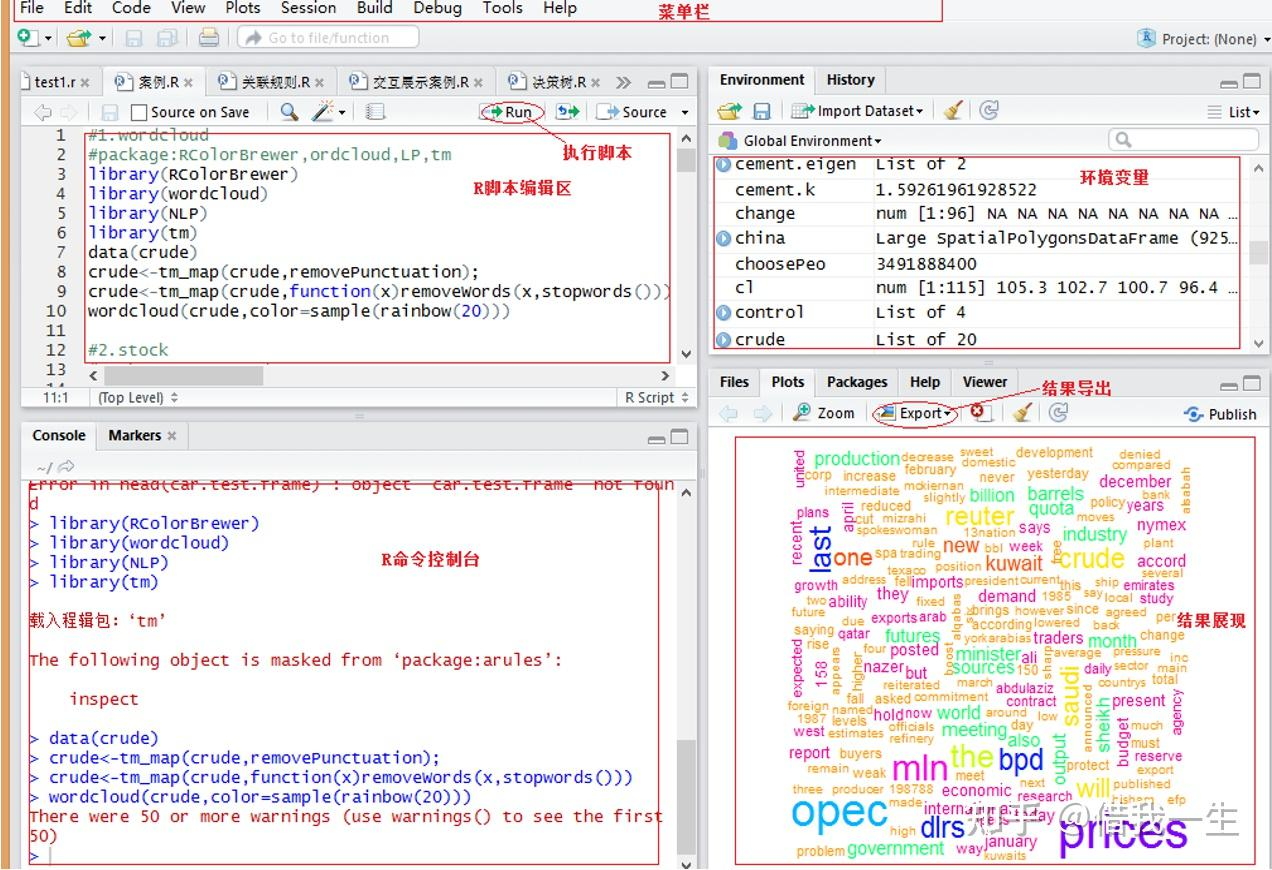
\includegraphics[width=1.0\textwidth]{Figure/Rstudio操作界面.jpg}
    \caption{R studio操作界面}
\end{figure}
\section{一个简单的示例(不是Hello World)}
\begin{lstlisting}[language=R, basicstyle=\ttfamily\small, backgroundcolor=\color{gray!10}, frame=leftline, xleftmargin=2em]
    # Listing 1.1 - A Sample R session
age <- c(1,3,5,2,11,9,3,9,12,3)
weight <- c(4.4,5.3,7.2,5.2,8.5,7.3,6.0,10.4,10.2,6.1)
mean(weight)
sd(weight)
cor(age,weight)
plot(age,weight)

\end{lstlisting}


\chapter{R语言预备知识}
\section{基本命令}
\subsection{获取工作目录}
使用$getwd()$函数获取当前工作目录，作用是查看当前工作目录在哪一个具体位置，C盘或者是其他,第一次使用可能会出现警告，但是也可以看到工作目录，你可以在运行一次代码，如下：
\begin{lstlisting}[language=R, basicstyle=\ttfamily\small, backgroundcolor=\color{gray!10}, frame=leftline, xleftmargin=2em]
> getwd()
[1] "C:/Users/橙/Documents"
Warning message:
In normalizePath(path.expand(path), winslash, mustWork) :
  path[1]="C:/Users/?/Documents": 文件名、目录名或卷标语法不正确。
> getwd()
[1] "C:/Users/橙/Documents"
\end{lstlisting}

\subsection{设置工作目录}
使用$setwd()$函数更改当前目录，把工作目录更改到你存放你需要使用的数据包的那个位置，更便于直接重工作目录中读取，否者需要使用全路径。在使用函数是需要几点注意，请看以下代码：
\begin{lstlisting}
> setwd("F:\R.cx")#工作目录的地址需要用双引号括起来，注意斜杠，这种单斜杠会报错
Error: '\R' is an unrecognized escape in character string starting ""F:\R"
> setwd("F:/R.cx")#这种单斜杠可以，能运行
> setwd("F://R.cx")#这行与下一行的双斜杠都行
> setwd("F:\\R.cx")
>
\end{lstlisting}

\subsection{注释}
R语言的注释使用\#号，写代码一定要常写注释，不然时间久了会忘记某代码的作用，便于后续操作。在Rstudio中可以使用Ctrl+shift+C经行多行注释。

\subsection{变量名的命名}
与其他语言的变量名命名差不多，主要要注意：数字不能开头；\%号是非法字符，不可以用来命名；.号后面不可以跟数字；不可以下划线开头。变量名可以为与你操作相关的名字命名，如我要对一行身高的数据求均值：
\begin{lstlisting}
higth<-c(175,169,179,175,180,183)
higth_mean<-mean(higth)#对身高求均值
\end{lstlisting}

\subsection{赋值}
R语言的赋值方式与其他语言有点区别，有三种，分别是左箭头<-（<键+-键（等号左边的那个，不要按Shift）），等号=，右箭头->，如：
\begin{lstlisting}
    > a<-2
> b=3
> c->4   #注意右箭头使用方法，被赋值的应该在右边，简单点说，就是某某赋值给谁，箭头就指向谁
Error in 4 <- c : invalid (do_set) left-hand side to assignment
> 4->c
> a      #键盘敲出变量名，回车后就会显示结果
[1] 2
> b
[1] 3
> c
[1] 4
>
\end{lstlisting}

\subsection{变量的显示}
1.命令行直接输入变量名\\

2.利用print()函数，如下
\begin{lstlisting}
> a<-2
> a     #命令行直接输入变量名
[1] 2
> print(a)     #利用print()函数
[1] 2
\end{lstlisting}

\subsection{查看与清除变量}
查看变量：$ls()$\\

清除指定变量：$rm()$\\

清除所有变量：$rm(list=ls())$ 如下：
\begin{lstlisting}
> ls()     #查看变量，这个函数是查看所有已定义的变量，输出所有变量名
[1] "a" "b" "c"
> rm(a)    #清除变量a
> rm(list=ls())    #清除所有变量 
\end{lstlisting}

\subsection{函数帮助文档查询}
当遇到一个函数不会用时，可以使用帮助文档查询，结果会在Rstudio的右下角框里显示，方法有三种：\\

1.?+要查询的函数\\

2.使用help()函数查询\\

3.使用example()函数查询\\

我以求和函数sum()为例：
\begin{lstlisting}
> ?sum
> help(sum)
> example(sum)    
\end{lstlisting}

\subsection{软件的退出与保存}
1.可以直接输入q()函数；也可以右上角直接叉掉，后根据提示操作\\

2.当写完一个文件时，可以点击保存按钮，根据提示选择保存位置，文件后缀有多种，看你保存哪种文件，有.R、.Rdata等后缀，.R一般是保存代码的，.Rdata是保存处理后的数据的。

\subsection{保存数据}
可以使用$save()$函数，可以保存多种格式的文件
\begin{lstlisting}
> save(b,file="xxx.Rdata") #保存b,文件是xxx，格式为.Rdata
> save(b,c,file="xxx.Rdata")  #保存b,c,文件是xxx，格式为.Rdata
> save.image("xxx.Rdata")  #保存所有（你定义的所有变量及数据），文件是xxx，格式为.Rdata    
\end{lstlisting}

\section{R语言语法}
\subsection{函数}
R中含有大量的函数，比如求和函数$sum()$，求均值$mean()$等直接可以拿来使用的函数，但是往往在实际操作过程中，因为需求不同需要自己写函数，就是自定义函数，类似于C或C++中的自定义函数，我们来看一下R中如何自定义函数,请看如下代码：
\begin{lstlisting}
>   #函数名<-function(){·······}
> f<-function(a,b)   #写一个求和函数,function()是固定格式
+ {
+   k<-a+b
+   return(k)      #返回结果为k，如果没有设置返回值，则函数会返回最后一行执行的结果
+ }
> f(3,4)            #使用函数名加一个括号调用函数
[1] 7
\end{lstlisting}
注：函数可以套函数使用

\subsubsection{输出函数}
$print()$函数，输出，与C语言中的$printf()$函数作用一样
\begin{lstlisting}
> print(5)
[1] 5    
\end{lstlisting}


\subsubsection{安装R包}
安装R包需要使用$install.packages()$或者$BiocManager::install()$函数安装，$library()$函数调用，以安装openxlsx为例，如下：
\begin{lstlisting}
安装R包代码如下
install.packages("openxlsx")
或BiocManager::install("openxlsx")
library(openxlsx)    
\end{lstlisting}
\subsubsection{文件的读取}

在 R 语言中，读取文件是数据分析的第一步。根据文件格式（txt, csv, xlsx）和数据结构的复杂度，我们可以选择不同的函数。以下是几种常用的读取函数及其参数详解：

\begin{enumerate}[label=\arabic*., leftmargin=2em]
    \item \textbf{scan() 函数}：适用于读取简单的数值、字符序列或大规模规则数据。
    \begin{itemize}
        \item \textbf{file}: 文件路径字符串。注意 Windows 路径需用 \texttt{"/"} 或 \texttt{"\\\\"}。
        \item \textbf{what}: 指定数据类型，如 \texttt{double()}, \texttt{integer()}, \texttt{character()}。
        \item \textbf{sep}: 分隔符，默认为空字符（空格、制表符、换行符均可）。
    \end{itemize}
\begin{lstlisting}[language=R, caption=scan函数示例]
# 读取纯数字
x <- scan(file = "data.txt", what = double())
# 读取混合类型（作为字符读入）
y <- scan(file = "mixed.txt", what = "")
\end{lstlisting}

    \item \textbf{readline() 函数}：主要用于交互式脚本，从控制台读取单行输入。
    \begin{itemize}
        \item \textbf{prompt}: 打印在终端的提示信息。
    \end{itemize}
\begin{lstlisting}[language=R]
name <- readline(prompt = "请输入您的姓名：")
print(paste("你好,", name))
\end{lstlisting}

    \item \textbf{readLines() 函数}：用于以“行”为单位读取文本文件。
    \begin{itemize}
        \item \textbf{n}: 读取的行数。
        \item \textbf{encoding}: 字符编码方式（如 \texttt{"UTF-8"}），解决中文乱码的关键。
    \end{itemize}
\begin{lstlisting}[language=R]
# 读取前三行内容
txt_content <- readLines("memo.txt", n = 3, encoding = "UTF-8")
\end{lstlisting}

    \item \textbf{read.table() 函数}：读取结构化表格数据的“万能钥匙”。
    \begin{itemize}
        \item \textbf{header}: 逻辑值，首行是否包含列名。
        \item \textbf{sep}: 字段分隔符。常见：\texttt{","} (CSV), \texttt{"\textbackslash t"} (Tab 间隔)。
        \item \textbf{na.strings}: 指定代表缺失值的字符。
    \end{itemize}
\begin{lstlisting}[language=R]
# 读取带有表头、逗号分隔、且将"999"视为缺失值的文件
my_data <- read.table("survey.txt", header = TRUE, sep = ",", na.strings = "999")
\end{lstlisting}

    \item \textbf{read.csv() 函数}：\texttt{read.table} 的变体，专为逗号分隔文件优化。
\begin{lstlisting}[language=R]
# 默认 header = TRUE
df <- read.csv("results.csv")
\end{lstlisting}

    \item \textbf{read.xlsx() 函数}：读取 Excel 文件的标准方案（需 \texttt{openxlsx} 包）。
\begin{lstlisting}[language=R]
library(openxlsx)
excel_data <- read.xlsx("report.xlsx", sheet = 1, startRow = 2)
\end{lstlisting}
\end{enumerate}

\paragraph{常用读取函数对比表}
\begin{table}[h]
\centering
\renewcommand{\arraystretch}{1.5}
\begin{tabular}{|l|l|l|l|}
\hline
\textbf{函数} & \textbf{主要用途} & \textbf{返回类型} & \textbf{适用场景} \\ \hline
\texttt{scan} & 快速读取元素 & 向量/列表 & 大规模数值或简单序列 \\ \hline
\texttt{readline} & 交互式输入 & 长度为1的字符向量 & 脚本运行中的人工干预 \\ \hline
\texttt{readLines} & 按行读取文本 & 字符向量 & 文本挖掘或非结构化数据 \\ \hline
\texttt{read.table} & 读取结构化表格 & 数据框 (data.frame) & 绝大多数实验原始数据 \\ \hline
\texttt{read.xlsx} & 读取Excel文件 & 数据框 (data.frame) & 现成的统计报表 \\ \hline
\end{tabular}
\end{table}

\paragraph{注意事项：}
在读取文件前，建议先使用 \texttt{getwd()} 查看当前工作目录，或使用 \texttt{setwd()} 设置路径，这样在 \texttt{file} 参数中只需写文件名即可，能极大简化代码。

\subsubsection{文件的输出}

在 R 语言中，将处理好的数据或结果保存到本地文件，主要使用以下几种函数：

\begin{enumerate}[label=\arabic*., leftmargin=2em]
    \item \textbf{write.table() 函数}：与 \texttt{read.table()} 对应，用于将数据框或矩阵输出为结构化文本文件。
    \begin{itemize}
        \item \textbf{x}: 要写入的对象。
        \item \textbf{file}: 保存路径。
        \item \textbf{append}: 逻辑值。若为 \texttt{TRUE}，则在原文件末尾追加；若为 \texttt{FALSE}，则覆盖原文件。
        \item \textbf{sep}: 分隔符，如 \texttt{sep = ","} 表示保存为 CSV 格式。
        \item \textbf{row.names/col.names}: 是否保留行名或列名（通常建议设为 \texttt{FALSE} 以保持纯净的数据格式）。
    \end{itemize}

    \item \textbf{write() 函数}：常用于将向量数据以特定列数写入文件。
\begin{lstlisting}[language=R]
# 将字符串写入桌面文件
write("Hello, world", "C:/Users/橙/Desktop/juli.txt")
\end{lstlisting}

    \item \textbf{cat() 函数}：功能强大的输出函数，可以将多个对象拼接并直接写入文件。
    \begin{itemize}
        \item \textbf{file}: 指定输出文件的路径。
        \item \textbf{append}: 控制写入模式。
        \begin{itemize}
            \item \texttt{append = TRUE} (或 \texttt{T}): \textbf{追加写入}，在文件原有内容后添加。
            \item \texttt{append = FALSE} (或缺省): \textbf{覆盖写入}，删除原文件内容并重新写入。
        \end{itemize}
    \end{itemize}
\begin{lstlisting}[language=R]
# 追加写入示例
cat("hello world", file="C:/Users/橙/Desktop/juli.txt", append=TRUE)

# 覆盖写入示例
cat("hello world", file="C:/Users/橙/Desktop/juli1.txt")
\end{lstlisting}

    \item \textbf{write.csv() 函数}：专用于输出逗号分隔文件的便捷函数。
    \begin{itemize}
        \item 默认 \texttt{sep = ","} 且 \texttt{col.names = TRUE}。
    \end{itemize}

    \item \textbf{save() / saveRDS() 函数}：用于保存 R 特有的二进制格式（.RData / .rds），适合保存模型或中间变量。
\end{enumerate}

\paragraph{输出函数对比总结}
\begin{table}[h]
\centering
\renewcommand{\arraystretch}{1.5}
\begin{tabular}{|l|l|l|}
\hline
\textbf{函数} & \textbf{输出对象类型} & \textbf{主要特点} \\ \hline
\texttt{write.table} & 数据框 / 矩阵 & 参数丰富，兼容性最强 \\ \hline
\texttt{write} & 向量 & 简单快捷，常用于简单列表 \\ \hline
\texttt{cat} & 字符串 / 拼接对象 & 灵活，支持追加/覆盖两种模式 \\ \hline
\texttt{write.csv} & 数据框 & 自动化设置，常用于 Excel 交互 \\ \hline
\end{tabular}
\end{table}

\paragraph{温馨提示：}
在输出数据到 CSV 时，若不想让第一列出现行索引数字，请务必加上参数 \texttt{row.names = FALSE}。

\subsection{向量 (Vector)}

向量是 R 语言中最基本的数据结构，其特点是所有元素必须属于同一类型（数值型、字符型或逻辑型）。

\begin{enumerate}[label=\arabic*., leftmargin=2em]
    \item \textbf{向量的创建}
    \begin{itemize}
        \item \textbf{c() 函数}：最常用的组合函数（combine），用于连接元素。
        \item \textbf{assign() 函数}：较少用，等同于赋值符号。
    \end{itemize}
\begin{lstlisting}[language=R]
x <- c(1, 3, 5, 7)          # 数值向量
y <- c("Apple", "Banana")   # 字符向量
assign("z", c(1, 2))        # 等同于 z <- c(1, 2)
\end{lstlisting}

    \item \textbf{创建等差序列}
    \begin{itemize}
        \item \textbf{冒号运算符 (:)}：生成步长为 1 的序列。
        \item \textbf{seq() 函数}：生成等差序列，可指定步长（by）或长度（length.out）。
        \item \textbf{rep() 函数}：生成重复序列。
    \end{itemize}
\begin{lstlisting}[language=R]
a <- 1:10                   # 1 到 10
b <- seq(from=1, to=10, by=2) # 1, 3, 5, 7, 9
c <- rep(1:3, times=2)      # 1, 2, 3, 1, 2, 3
d <- rep(1:3, each=2)       # 1, 1, 2, 2, 3, 3
\end{lstlisting}

    \item \textbf{向量的索引 (Indexing)}
    R 的索引从 \textbf{1} 开始，这与 Python/C 不同。
    \begin{itemize}
        \item \textbf{正整数索引}：提取对应位置元素。
        \item \textbf{负整数索引}：\textbf{剔除}对应位置元素。
        \item \textbf{逻辑索引}：提取满足条件（TRUE）的元素。
        \item \textbf{名称索引}：若向量有 \texttt{names}，可按名提取。
    \end{itemize}
\begin{lstlisting}[language=R]
v <- c(10, 20, 30, 40, 50)
v[2]          # 提取第2个: 20
v[c(1, 3)]    # 提取第1和第3个: 10, 30
v[-1]         # 剔除第1个: 20, 30, 40, 50
v[v > 35]     # 提取大于35的: 40, 50
\end{lstlisting}
    \item \textbf{向量元素的更改}
    通过索引选中特定位置的元素，并使用赋值符号 \texttt{<-} 将新值赋给它。
\begin{lstlisting}[language=R]
v <- c(10, 20, 30, 40)
v[2] <- 200            # 将第2个元素修改为 200
v[v < 35] <- 0         # 将所有小于 35 的元素统一修改为 0
v[c(1, 3)] <- c(8, 9)  # 同时修改第1和第3个元素
\end{lstlisting}

    \item \textbf{向量元素的删除}
    R 语言中“删除”元素的本质是：\textbf{创建一个不包含该元素的新向量}并覆盖原变量。
    \begin{itemize}
        \item \textbf{按位置删除}：使用负索引。
        \item \textbf{按值删除}：利用逻辑判断结合 \texttt{!=}（不等于）或 \texttt{\%in\%}（包含于）。
        \item \textbf{全部清空}：将变量赋值为 \texttt{NULL}。
    \end{itemize}
\begin{lstlisting}[language=R]
v <- c("A", "B", "C", "D", "E")

# 1. 删除特定位置元素
v <- v[-2]             # 删除第2个元素 "B"
v <- v[-c(1, 3)]       # 同时删除此时的第1和第3个元素

# 2. 按值删除
v <- v[v != "E"]       # 提取所有不等于 "E" 的元素，达到删除 "E" 的效果

# 3. 删除特定范围的元素
nums <- 1:10
nums <- nums[!(nums %in% c(2, 4, 6))] # 删除 2, 4, 6
\end{lstlisting}

    \item \textbf{向量的扩展}
    可以通过为超出当前长度的索引赋值来动态扩展向量。
\begin{lstlisting}[language=R]
v <- c(1, 2)
v[4] <- 10             # v 变为 c(1, 2, NA, 10)，中间会自动补 NA
\end{lstlisting}
    \item \textbf{向量化运算 (Vectorized Operation)}
    R 的一大特色是运算符会作用于向量的每一个元素。
\begin{lstlisting}[language=R]
x <- c(1, 2, 3)
y <- c(10, 20, 30)
x + y         # 结果: 11, 22, 33
x * 2         # 结果: 2, 4, 6
\end{lstlisting}
\end{enumerate}



\paragraph{常用向量函数汇总表}
\begin{table}[h]
\centering
\renewcommand{\arraystretch}{1.4}
\small % 适当缩小字体以容纳更多内容
\begin{tabular}{|l|l|p{7cm}|}
\hline
\textbf{类别} & \textbf{函数} & \textbf{功能说明} \\ \hline
\multirow{3}{*}{\textbf{属性查询}} & \texttt{length(x)} & 返回向量的长度（元素个数） \\ \cline{2-3} 
 & \texttt{mode(x)} & 返回向量的数据类型（如 numeric, character） \\ \cline{2-3} 
 & \texttt{names(x)} & 获取或设置向量元素的名称 \\ \hline
\multirow{4}{*}{\textbf{统计汇总}} & \texttt{sum(x)} & 向量元素求和 \\ \cline{2-3} 
 & \texttt{mean(x)} & 向量元素求平均值 \\ \cline{2-3} 
 & \texttt{max(x) / min(x)} & 返回向量中的最大值 / 最小值 \\ \cline{2-3} 
 & \texttt{sd(x) / var(x)} & 返回向量的标准差 / 方差 \\ \hline
\multirow{4}{*}{\textbf{排序与转换}} & \texttt{sort(x)} & 对向量进行排序（默认为升序） \\ \cline{2-3} 
 & \texttt{rev(x)} & 将向量元素完全反转 \\ \cline{2-3} 
 & \texttt{unique(x)} & 去除向量中的重复元素，仅保留唯一的项 \\ \cline{2-3} 
 & \texttt{order(x)} & 返回排序后的元素在原向量中的索引位置 \\ \hline
\multirow{4}{*}{\textbf{搜索与逻辑}} & \texttt{which(x == a)} & 返回符合条件 \texttt{a} 的元素下标（位置） \\ \cline{2-3} 
 & \texttt{which.max(x)} & 返回最大值所在的第一个位置索引 \\ \cline{2-3} 
 & \texttt{is.na(x)} & 检测缺失值，返回逻辑向量（TRUE/FALSE） \\ \cline{2-3} 
 & \texttt{any() / all()} & 判断向量中是否存在 / 是否全部为 TRUE \\ \hline
\multirow{2}{*}{\textbf{数据清洗}} & \texttt{na.omit(x)} & 移除向量中的所有缺失值 (\texttt{NA}) \\ \cline{2-3} 
 & \texttt{round(x, n)} & 将数值四舍五入保留 \texttt{n} 位小数 \\ \hline
\end{tabular}
\end{table}

\paragraph{注意事项：}
如果将不同类型的数据放入同一个向量，R 会进行“隐式转换”（Coercion），转换顺序通常为：\texttt{Logical < Integer < Double < Character}。例如 \texttt{c(1, "A")} 会导致 1 被转换为字符型 \texttt{"1"}。

\subsection{NA 与 NULL 值}

在 R 语言中，\texttt{NA} 和 \texttt{NULL} 都有“空”的含义，但在处理逻辑和数据结构中有着本质的区别。

\begin{enumerate}[label=\arabic*., leftmargin=2em]
    \item \textbf{NA (Not Available)}
    \texttt{NA} 表示内容缺失。它是一个“占位符”，代表该位置应该有值，但目前不知道是多少。
    \begin{itemize}
        \item \textbf{特点}：\texttt{NA} 具有长度（长度为 1），且有类型之分（如 \texttt{NA\_integer\_}, \texttt{NA\_character\_}）。
        \item \textbf{逻辑运算}：任何与 \texttt{NA} 进行的算术运算结果通常仍为 \texttt{NA}（例如 \texttt{1 + NA = NA}）。
    \end{itemize}

    \item \textbf{NULL (Null Object)}
    \texttt{NULL} 代表一个空对象。它表示“什么都没有”，连占位符都不是。
    \begin{itemize}
        \item \textbf{特点}：\texttt{NULL} 的长度始终为 0，不占用向量空间。
        \item \textbf{用途}：常用于初始化一个空变量，或者从列表（List）中彻底删除某个元素。
    \end{itemize}

    \item \textbf{常用检测与处理函数}
    注意：\texttt{NA} 不能使用 \texttt{==} 进行判断，必须使用专用函数 \texttt{is.na()}。
\begin{lstlisting}[language=R]
x <- c(1, 2, NA, 4)
is.na(x)          # 返回逻辑向量: FALSE FALSE TRUE FALSE
anyNA(x)          # 快速检查是否存在缺失值: TRUE

y <- NULL
is.null(y)        # 检查是否为NULL: TRUE
\end{lstlisting}

    \item \textbf{向量中的行为对比}
    这是理解两者差异最直观的方式：
\begin{lstlisting}[language=R]
# NA 占据位置，作为元素存在
v_na <- c(1, NA, 3)
length(v_na)      # 结果为 3

# NULL 不占位置（在组合时被忽略）
v_null <- c(1, NULL, 3)
length(v_null)    # 结果为 2
\end{lstlisting}
\end{enumerate}



\paragraph{NA 与 NULL 核心差异表}
\begin{table}[h]
\centering
\renewcommand{\arraystretch}{1.5}
\begin{tabular}{|l|p{5cm}|p{5cm}|}
\hline
\textbf{维度} & \textbf{NA (缺失值)} & \textbf{NULL (空对象)} \\ \hline
\textbf{含义} & 存在但未知 (Missing value) & 不存在该对象 (Undefined) \\ \hline
\textbf{长度} & 1 & 0 \\ \hline
\textbf{类型示例} & \texttt{NA\_integer\_}, \texttt{NA\_character\_} & 唯一的 \texttt{NULL} 类 \\ \hline
\textbf{运算} & \texttt{1 + NA = NA} & \texttt{1 + NULL = numeric(0)} \\ \hline
\textbf{检测函数} & \texttt{is.na()} & \texttt{is.null()} \\ \hline
\textbf{数据框行为} & 在表格中显示为单元格空白/NA & 无法作为独立列存在 \\ \hline
\end{tabular}
\end{table}

\paragraph{进阶提示：}
在进行统计计算（如 \texttt{sum()}, \texttt{mean()}）时，如果向量包含 \texttt{NA}，结果默认会变成 \texttt{NA}。此时需要显式设置参数 \texttt{na.rm = TRUE} 来剔除缺失值后再计算：\texttt{mean(x, na.rm = TRUE)}。

\subsection{矩阵 (Matrix)}

矩阵是一个二维的数据结构，可以看作是排列成行和列的向量。

\begin{enumerate}[label=\arabic*., leftmargin=2em]
    \item \textbf{矩阵的创建}
    使用 \texttt{matrix()} 函数，通过指定数据向量、行数或列数来创建。
    \begin{itemize}
        \item \textbf{data}: 包含矩阵元素的向量。
        \item \textbf{nrow / ncol}: 设定的行数和列数。
        \item \textbf{byrow}: 逻辑值。若为 \texttt{TRUE}，则按行填充数据；默认为 \texttt{FALSE}（按列填充）。
    \end{itemize}
\begin{lstlisting}[language=R]
# 创建一个 2 行 3 列的矩阵
m1 <- matrix(1:6, nrow = 2, ncol = 3)
# 按行填充
m2 <- matrix(1:6, nrow = 2, byrow = TRUE)
\end{lstlisting}

    \item \textbf{矩阵的合并与维度命名}
    \begin{itemize}
        \item \textbf{rbind()}: 将多个向量或矩阵按\textbf{行}合并。
        \item \textbf{cbind()}: 将多个向量或矩阵按\textbf{列}合并。
        \item \textbf{dimnames}: 设置行名和列名。
    \end{itemize}
\begin{lstlisting}[language=R]
v1 <- c(1, 2); v2 <- c(3, 4)
m_row <- rbind(v1, v2)  # 2行2列
colnames(m_row) <- c("Col1", "Col2")
rownames(m_row) <- c("Row1", "Row2")
\end{lstlisting}

    \item \textbf{矩阵的索引 (Indexing)}
    使用 \texttt{[行索引, 列索引]} 的格式。
\begin{lstlisting}[language=R]
m <- matrix(1:9, nrow = 3)
m[1, 2]     # 提取第 1 行第 2 列的元素
m[1, ]      # 提取第 1 行所有元素（返回向量）
m[, 2:3]    # 提取第 2 到 3 列所有元素
m[-1, ]     # 删除第 1 行后的剩余部分
\end{lstlisting}

    \item \textbf{常用矩阵运算函数}
    矩阵运算在 R 中非常高效。
\begin{lstlisting}[language=R]
t(m)        # 矩阵转置
diag(m)     # 提取对角线元素
m * m       # 元素级乘法（对应位置相乘）
m %*% m     # 线性代数中的矩阵乘法
colSums(m)  # 对每一列求和
rowMeans(m) # 对每一行求平均值
\end{lstlisting}
\end{enumerate}



\paragraph{矩阵核心属性函数表}
\begin{table}[h]
\centering
\renewcommand{\arraystretch}{1.5}
\begin{tabular}{|l|l|l|}
\hline
\textbf{函数} & \textbf{功能说明} & \textbf{返回值示例} \\ \hline
\texttt{dim(m)} & 获取矩阵的维度（行数和列数） & \texttt{c(nrow, ncol)} \\ \hline
\texttt{nrow(m)} & 单独获取行数 & 整数 \\ \hline
\texttt{ncol(m)} & 单独获取列数 & 整数 \\ \hline
\texttt{attributes(m)} & 查看矩阵的所有元数据（如维度、行列名） & 列表 \\ \hline
\end{tabular}
\end{table}

\paragraph{进阶提示：}
1. 如果对矩阵进行索引时只取一行或一列，结果默认会退化（Drop）为向量。如果不希望退化，请使用 \texttt{m[1, , drop = FALSE]}。
2. 矩阵本质上是一个带有维度属性（\texttt{dim}）的向量，因此 \texttt{length(m)} 返回的是矩阵中元素的总个数。

\subsection{列表 (List)}

列表是 R 语言中最复杂的数据结构，它可以包含不同类型的对象，且对象之间的长度可以不同。

\begin{enumerate}[label=\arabic*., leftmargin=2em]
    \item \textbf{列表的创建}
    使用 \texttt{list()} 函数创建，建议在创建时为每个成分命名，方便后续调用。
\begin{lstlisting}[language=R]
# 创建包含向量、矩阵和字符串的列表
my_list <- list(
    vec = c(1, 2, 3), 
    mat = matrix(1:4, nrow = 2), 
    msg = "Hello R"
)
\end{lstlisting}

    \item \textbf{列表的索引 (关键点)}
    访问列表元素有两种常用的方式，其返回结果完全不同：
    \begin{itemize}
        \item \textbf{单方括号 \texttt{[ ]}}：提取列表的**子集**，结果仍为一个“小列表”。
        \item \textbf{双方括号 \texttt{[[ ]}}：提取列表中的**具体内容**，结果为该位置原始的对象类型。
        \item \textbf{美元符号 \texttt{\$}}：按名称提取内容，效果等同于 \texttt{[[ ]]}。
    \end{itemize}
\begin{lstlisting}[language=R]
my_list[1]      # 返回一个只含向量的列表
my_list[[1]]    # 返回具体的数值向量: 1, 2, 3
my_list$vec     # 同上，返回数值向量
\end{lstlisting}

    \item \textbf{列表元素的更改与添加}
\begin{lstlisting}[language=R]
# 修改元素
my_list[[3]] <- "Goodbye" 

# 添加新元素
my_list$new_item <- c(TRUE, FALSE)

# 删除元素：赋值为 NULL
my_list$msg <- NULL
\end{lstlisting}

    \item \textbf{列表的合并与转换}
\begin{lstlisting}[language=R]
# 合并列表
combined_list <- c(list1, list2)

# 将列表转换为向量（若类型一致）
v <- unlist(my_list) 
\end{lstlisting}
\end{enumerate}



\paragraph{列表核心操作汇总表}
\begin{table}[h]
\centering
\renewcommand{\arraystretch}{1.5}
\begin{tabular}{|l|l|p{7cm}|}
\hline
\textbf{操作} & \textbf{语法} & \textbf{结果说明} \\ \hline
\texttt{提取子集} & \texttt{L[i]} & 返回一个列表，包含第 \texttt{i} 个元素 \\ \hline
\texttt{提取内容} & \texttt{L[[i]]} & 返回第 \texttt{i} 个元素本身的类型（向量/矩阵等） \\ \hline
\texttt{按名提取} & \texttt{L\$name} & 与 \texttt{L[["name"]]} 等价，最常用的方式 \\ \hline
\texttt{元素个数} & \texttt{length(L)} & 返回列表中顶层成分的数量 \\ \hline
\texttt{查看结构} & \texttt{str(L)} & \textbf{极其重要}：显示列表的层级和内容结构 \\ \hline
\end{tabular}
\end{table}

\paragraph{进阶提示：}
1. \textbf{为什么需要双括号？} 想象列表是一个装着许多盒子的货车，\texttt{L[1]} 是卸下了第一辆货车上的第一个“盒子”，而 \texttt{L[[1]]} 则是打开了盒子，拿到了里面的“货物”。
2. \textbf{str() 函数}：面对复杂的统计模型输出结果（通常是多层嵌套列表），使用 \texttt{str()} 是理清数据脉络的第一步。

\subsection{数据框 (Data Frame)}

数据框是 R 中最常用的数据结构，用于存储表格状数据。

\begin{enumerate}[label=\arabic*., leftmargin=2em]
    \item \textbf{数据框的创建}
    使用 \texttt{data.frame()} 函数，将多个向量组合成列。
\begin{lstlisting}[language=R]
# 创建一个包含病患信息的数据框
patient_id <- c(101, 102, 103)
age <- c(25, 42, 37)
treatment <- c("A", "B", "A")

df <- data.frame(ID = patient_id, Age = age, Group = treatment)
\end{lstlisting}

    \item \textbf{查看数据框属性}
    对于大型数据集，直接输入变量名查看是不现实的。
    \begin{itemize}
        \item \textbf{head(df, n)}: 查看前 n 行（默认为 6 行）。
        \item \textbf{tail(df, n)}: 查看后 n 行。
        \item \textbf{dim(df)}: 获取行数和列数。
        \item \textbf{str(df)}: 查看数据框结构（各列类型及前几个值）。
        \item \textbf{summary(df)}: 获取每列的统计摘要（最大、最小、均值等）。
    \end{itemize}

    \item \textbf{数据框的索引与提取}
\begin{lstlisting}[language=R]
# 1. 访问列
df$Age           # 返回 Age 列的向量
df[["Age"]]      # 同上
df[, 2]          # 提取第 2 列

# 2. 访问行
df[1, ]          # 提取第 1 行

# 3. 逻辑筛选（极其常用）
# 提取 Group 为 "A" 的所有病患行
group_a <- df[df$Group == "A", ]
\end{lstlisting}

    \item \textbf{数据框的修改与合并}
\begin{lstlisting}[language=R]
# 添加新列
df$Gender <- c("M", "F", "M")

# 修改列名
colnames(df)[3] <- "Treatment_Group"

# 合并
# rbind(df1, df2) 合并行（列名需一致）
# cbind(df1, df2) 合并列（行数需一致）
\end{lstlisting}
\end{enumerate}



\paragraph{数据框处理常用函数表}
\begin{table}[h]
\centering
\renewcommand{\arraystretch}{1.5}
\begin{tabular}{|l|l|l|}
\hline
\textbf{函数} & \textbf{功能说明} & \textbf{备注} \\ \hline
\texttt{nrow(df)} & 返回行数 & 对应观察对象数 \\ \hline
\texttt{ncol(df)} & 返回列数 & 对应变量数 \\ \hline
\texttt{names(df)} & 获取列名 & 等价于 \texttt{colnames()} \\ \hline
\texttt{subset()} & 按条件提取子集 & \texttt{subset(df, Age > 30)} \\ \hline
\texttt{with()} & 简化列名引用 & \texttt{with(df, mean(Age))} \\ \hline
\end{tabular}
\end{table}

\paragraph{进阶提示：}
1. \textbf{字符与因子}：在旧版 R 中，创建数据框时字符会自动转为因子（Factor）。现代版本（R 4.0+）默认不再转换。若需手动控制，可设置 \texttt{stringsAsFactors = TRUE}。
2. \textbf{缺失值处理}：使用 \texttt{na.omit(df)} 可以快速删除数据框中所有包含 \texttt{NA} 的行。



\subsection{因子 (Factor)}

因子用于存储分类变量。在 R 内部，因子被存储为整数向量，并带有一个标签（Label）向量。

\begin{enumerate}[label=\arabic*., leftmargin=2em]
    \item \textbf{因子的创建}
    使用 \texttt{factor()} 函数。
    \begin{itemize}
        \item \textbf{levels}: 手动指定分类的水平。如果不指定，R 会按字母顺序排列。
        \item \textbf{labels}: 为水平设置更直观的标签。
    \end{itemize}
\begin{lstlisting}[language=R]
# 创建简单因子
gender <- factor(c("Male", "Female", "Female", "Male"))
# 查看因子水平
levels(gender) # 结果为 "Female" "Male"
\end{lstlisting}

    \item \textbf{有序因子 (Ordered Factor)}
    用于有明显等级顺序的数据（如：病情的轻、中、重）。
\begin{lstlisting}[language=R]
status <- c("Low", "High", "Medium", "High", "Low")
# 指定等级顺序，否则默认按字母排序 (High, Low, Medium)
status_factor <- factor(status, 
                        ordered = TRUE, 
                        levels = c("Low", "Medium", "High"))
\end{lstlisting}

    \item \textbf{常用函数与操作}
\begin{lstlisting}[language=R]
# 1. 频数统计
table(gender)     # 统计每个水平出现的次数

# 2. 修改因子水平
levels(gender) <- c("F", "M") # 将 Female/Male 简写

# 3. 将连续变量因子化 (分组)
age <- c(22, 45, 18, 65, 30)
age_group <- cut(age, breaks = c(0, 18, 60, Inf), 
                 labels = c("Minor", "Adult", "Senior"))
\end{lstlisting}
\end{enumerate}



\paragraph{因子相关常用函数表}
\begin{table}[h]
\centering
\renewcommand{\arraystretch}{1.5}
\begin{tabular}{|l|l|l|}
\hline
\textbf{函数} & \textbf{功能说明} & \textbf{备注} \\ \hline
\texttt{is.factor()} & 检查对象是否为因子 & 返回逻辑值 \\ \hline
\texttt{levels()} & 获取或设置因子的水平 & 返回字符向量 \\ \hline
\texttt{nlevels()} & 返回因子的水平个数 & 等价于 \texttt{length(levels())} \\ \hline
\texttt{as.factor()} & 将其他类型强制转换为因子 & 不支持指定顺序 \\ \hline
\texttt{gl()} & 生成规则的因子序列 & \texttt{gl(n, k)} 生成n个水平,每水平重复k次 \\ \hline
\end{tabular}
\end{table}

\paragraph{进阶提示：数值型因子的“陷阱”}
如果一个因子是由数字组成的（例如 \texttt{f <- factor(c(10, 20, 30))}），直接使用 \texttt{as.numeric(f)} 会返回其内部的**层级索引**（1, 2, 3）而不是原本的数字。
\textbf{正确转换方法：} \texttt{as.numeric(as.character(f))}。

\subsection{常用数学与统计函数}

R 语言内置了极其丰富的数学与统计工具，能够高效处理向量化数据。

\begin{enumerate}[label=\arabic*., leftmargin=2em]
    \item \textbf{基本数学函数}
    这些函数通常作用于向量中的每一个元素。
\begin{lstlisting}[language=R]
abs(-5)           # 绝对值: 5
sqrt(16)          # 开平方: 4
exp(1)            # 指数函数: 2.718...
log(100, base=10) # 对数函数，默认以 e 为底
round(3.1415, 2)  # 四舍五入保留两位小数: 3.14
ceiling(3.1)      # 向上取整: 4
floor(3.9)        # 向下取整: 3
\end{lstlisting}

    \item \textbf{统计汇总函数}
    用于描述性统计分析。注意：若数据中包含 \texttt{NA}，需添加 \texttt{na.rm = TRUE}。
\begin{lstlisting}[language=R]
x <- c(1, 5, 10, 20, NA)
sum(x, na.rm = TRUE)    # 求和
mean(x, na.rm = TRUE)   # 算术平均值
median(x, na.rm = TRUE) # 中位数
var(x, na.rm = TRUE)    # 方差
sd(x, na.rm = TRUE)     # 标准差
range(x, na.rm = TRUE)  # 极差（返回最小值和最大值）
quantile(x, 0.75, na.rm = TRUE) # 计算 75% 分位数
\end{lstlisting}

    \item \textbf{概率分布函数 (以正态分布为例)}
    R 中对每种分布都有四类函数，其前缀分别为：
    \begin{itemize}
        \item \textbf{d} (density): 密度函数 / 概率质量函数。
        \item \textbf{p} (probability): 累积分布函数（左尾概率）。
        \item \textbf{q} (quantile): 分位数函数（\texttt{p} 的反函数）。
        \item \textbf{r} (random): 生成符合该分布的随机数。
    \end{itemize}
\begin{lstlisting}[language=R]
rnorm(100, mean = 0, sd = 1)  # 生成 100 个标准正态分布随机数
pnorm(1.96)                   # 标准正态分布下，Z < 1.96 的概率 (约 0.975)
qnorm(0.95)                   # 找到对应 95% 累积概率的 Z 值 (约 1.64)
\end{lstlisting}
\end{enumerate}



\paragraph{常用分布函数名对照表}
\begin{table}[h]
\centering
\renewcommand{\arraystretch}{1.5}
\begin{tabular}{|l|l|l|}
\hline
\textbf{分布类型} & \textbf{R 函数名后缀} & \textbf{典型应用场景} \\ \hline
正态分布 (Normal) & \texttt{norm} & 绝大多数连续变量分析 \\ \hline
T 分布 (Student's t) & \texttt{t} & 小样本均值检验 \\ \hline
二项分布 (Binomial) & \texttt{binom} & 患病/未患病等二分类实验 \\ \hline
泊松分布 (Poisson) & \texttt{pois} & 罕见事件发生次数统计 \\ \hline
卡方分布 (Chi-squared) & \texttt{chisq} & 计数资料的关联性检验 \\ \hline
\end{tabular}
\end{table}

\paragraph{进阶提示：}
在进行统计绘图或模拟实验时，如果希望结果具有可重复性，请务必在生成随机数前使用 \texttt{set.seed(数值)} 函数设置随机数种子（如 \texttt{set.seed(123)}）。


\section{控制流与自定义函数}

控制流用于管理代码的执行逻辑，而函数则将一系列操作封装成一个可重复调用的单元。

\begin{enumerate}[label=\arabic*., leftmargin=2em]
    \item \textbf{条件判断 (If-Else)}
    用于根据逻辑条件的真假执行不同的代码块。
\begin{lstlisting}[language=R]
x <- 85
if (x >= 90) {
    print("优秀")
} else if (x >= 60) {
    print("合格")
} else {
    print("不合格")
}

# 向量化版本：ifelse() 函数 (极其常用)
# 语法：ifelse(test, yes, no)
status <- ifelse(x >= 60, "Pass", "Fail")
\end{lstlisting}

    \item \textbf{循环结构 (Loop)}
    \begin{itemize}
        \item \textbf{for 循环}：遍历向量或列表中的每一个元素。
        \item \textbf{while 循环}：当条件满足时持续运行。
    \end{itemize}
\begin{lstlisting}[language=R]
# for 循环示例
for (i in 1:5) {
    print(i^2)
}

# 批量处理文件名示例
files <- c("sample1.csv", "sample2.csv")
for (f in files) {
    # data <- read.csv(f)
    # ... 处理代码 ...
}
\end{lstlisting}

    \item \textbf{自定义函数 (Function)}
    函数允许你将复杂的逻辑打包。R 函数会自动返回最后一行表达式的结果。
\begin{lstlisting}[language=R]
# 定义函数语法：函数名 <- function(参数1, 参数2, ...) { 逻辑体 }
calc_bmi <- function(weight, height) {
    bmi <- weight / (height^2)
    return(bmi) # 显式返回，也可以省略直接写 bmi
}

# 调用函数
my_bmi <- calc_bmi(70, 1.75)
\end{lstlisting}
\end{enumerate}



\paragraph{控制流常用关键字与技巧表}
\begin{table}[h]
\centering
\renewcommand{\arraystretch}{1.5}
\begin{tabular}{|l|l|l|}
\hline
\textbf{关键字} & \textbf{功能说明} & \textbf{应用场景} \\ \hline
\texttt{if / else} & 标准条件分支 & 针对单个逻辑判断 \\ \hline
\texttt{ifelse()} & 向量化条件判断 & \textbf{推荐}：用于对数据框整列进行分类 \\ \hline
\texttt{for} & 固定次数循环 & 遍历已知长度的对象 \\ \hline
\texttt{break} & 强制跳出当前循环 & 满足特定错误或条件时停止 \\ \hline
\texttt{next} & 跳过本次循环，进入下一次 & 过滤不符合条件的样本 \\ \hline
\texttt{return()} & 指定函数返回值 & 提前结束函数或明确输出结果 \\ \hline
\end{tabular}
\end{table}

\paragraph{进阶提示：避免“显式循环”}
R 语言是向量化语言。在处理大型数据框时，尽量使用 \texttt{ifelse()} 或 \texttt{apply} 系列函数（如 \texttt{lapply}, \texttt{sapply}），而不是直接写 \texttt{for} 循环。这不仅能让代码更简洁，还能显著提升运行速度。
\chapter{数据分析}
\section{数据清洗与转换 (dplyr \& tidyr)}

在 R 语言的实际应用中，原始数据往往是“脏”的或格式不规范的。\texttt{tidyverse} 生态系统中的 \texttt{dplyr} 和 \texttt{tidyr} 提供了一套高度一致、语义化的工具。

\subsection{dplyr 的核心动作 (Verbs)}
\texttt{dplyr} 包通过几个核心动词函数，覆盖了大部分数据转换需求：

\begin{enumerate}[label=\arabic*., leftmargin=2em]
    \item \textbf{filter()}：按行筛选数据。
    \item \textbf{select()}：按列选取变量。
    \item \textbf{mutate()}：衍生新列。
    \item \textbf{arrange()}：数据排序。
    % 修正点：将 group_by 写在 \texttt{} 中并转义下划线
    \item \textbf{\texttt{group\_by()}} 与 \textbf{\texttt{summarise()}}：分组聚合。
\end{enumerate}

\subsection{tidyr 的数据重塑}
% 修正点：对 pivot_longer 和 pivot_wider 进行转义
\begin{itemize}
    \item \texttt{pivot\_longer()}：将宽格式数据转换为长格式。
    \item \texttt{pivot\_wider()}：将长格式数据转换为宽格式。
\end{itemize}



\subsection{常用清洗函数对比总结}
\begin{table}[h!]
\centering
\renewcommand{\arraystretch}{1.5}
\begin{tabular}{|l|p{6cm}|l|}
\hline
\textbf{函数} & \textbf{功能描述} & \textbf{SQL/Excel 对应} \\ \hline
\texttt{filter()} & 筛选满足条件的观察行 & Filter / WHERE \\ \hline
\texttt{select()} & 选取或剔除指定的变量列 & Select / Column hide \\ \hline
\texttt{mutate()} & 新增列并保留原数据 & Calculated Field \\ \hline
% 修正点：表格中的下划线处理
\texttt{group\_by()} & 将数据按类别分组 & GROUP BY \\ \hline
\texttt{summarise()} & 将多行数据压缩为一行汇总结果 & Pivot Table / Sum \\ \hline
\texttt{inner\_join()} & 根据键值合并两个数据框 & VLOOKUP / JOIN \\ \hline
\end{tabular}
\end{table}





\section{数据可视化 (ggplot2)}

\texttt{ggplot2} 是 R 语言中最强大的可视化包。其核心逻辑是通过加号 (\texttt{+}) 将不同的图层叠加在一起。

\subsection{ggplot2 的基础语法结构}
一个基本的绘图模板如下：
\begin{lstlisting}[language=R]
ggplot(data = <DATA>) + 
  <GEOM_FUNCTION>(mapping = aes(<MAPPINGS>)) +
  <THEME_FUNCTION>()
\end{lstlisting}

\begin{enumerate}[label=\arabic*., leftmargin=2em]
    \item \textbf{数据 (Data)}：必须是一个数据框 (\texttt{data.frame})。
    \item \textbf{映射 (Mapping)}：使用 \texttt{aes()} 函数定义，指定变量如何映射到视觉属性（如 \texttt{x} 轴、\texttt{y} 轴、颜色 \texttt{color}、形状 \texttt{shape}）。
    \item \textbf{几何对象 (Geoms)}：决定图表类型（点、线、柱等）。
\end{enumerate}



\subsection{常见图表类型 (Geoms)}
根据研究目的选择不同的几何对象函数：

\begin{itemize}
    \item \textbf{散点图}：\texttt{geom\_point()} —— 用于观察两个连续变量的关系。
    \item \textbf{箱线图}：\texttt{geom\_boxplot()} —— 用于观察变量的分布及异常值。
    \item \textbf{条形图}：\texttt{geom\_bar()} 或 \texttt{geom\_col()} —— 用于展示分类数据的频数或数值。
    \item \textbf{折线图}：\texttt{geom\_line()} —— 常用于时间序列数据。
    \item \textbf{直方图}：\texttt{geom\_histogram()} —— 观察单变量的分布密度。
\end{itemize}

\subsection{图形美化：颜色、标签与主题}
通过叠加额外的图层，可以让图表达到出版标准。
\begin{lstlisting}[language=R]
df %>%
  ggplot(aes(x = weight, y = height, color = group)) +
  geom_point(size = 3, alpha = 0.7) +
  labs(
    title = "Weight vs Height",
    x = "Weight (kg)",
    y = "Height (cm)",
    color = "Group Name"
  ) +
  theme_bw() # 使用经典白底黑框主题
\end{lstlisting}

\subsection{分面 (Faceting)}
分面是 \texttt{ggplot2} 最强大的功能之一，可以根据某个分类变量快速生成多张子图。
\begin{itemize}
    \item \texttt{facet\_wrap(\~{}variable)}：按一个变量自动排列子图。
    \item \texttt{facet\_grid(rows \~{} cols)}：按行和列两个变量生成矩阵子图。
\end{itemize}



\subsection{常用外观调整函数对照表}
\begin{table}[h!]
\centering
\renewcommand{\arraystretch}{1.5}
\begin{tabular}{|l|l|p{6cm}|}
\hline
\textbf{类别} & \textbf{函数} & \textbf{功能说明} \\ \hline
\texttt{坐标轴范围} & \texttt{xlim(), ylim()} & 设置 X 或 Y 轴的起止点 \\ \hline
\texttt{颜色比例} & \texttt{scale\_color\_manual()} & 手动指定离散变量的颜色（如实验组红色，对照组蓝色） \\ \hline
\texttt{坐标翻转} & \texttt{coord\_flip()} & 将 X 轴与 Y 轴对调（常用于条形图） \\ \hline
\texttt{预设主题} & \texttt{theme\_minimal()} & 极简主题，去除冗余网格线 \\ \hline
\texttt{保存图表} & \texttt{ggsave()} & 将最后生成的图表保存为 pdf, png 或 tiff 格式 \\ \hline
\end{tabular}
\end{table}

\paragraph{注意事项：}
1. 注意 \texttt{color}（轮廓色/点色）与 \texttt{fill}（填充色）的区别。柱状图的颜色通常使用 \texttt{fill}。
2. 多个图层之间必须使用 \texttt{+} 连接，且 \texttt{+} 必须写在行末，不能写在行首。
3. 如果在 \texttt{aes()} 内部设置颜色，它是根据数据自动映射；如果在 \texttt{aes()} 外部设置颜色（如 \texttt{geom\_point(color = "blue")}），则是统一指定颜色。



\section{统计检验基础}

R 语言提供了强大的内置函数，用于执行常见的参数化与非参数化检验。在执行检验前，通常需要确保数据满足正态性（\texttt{shapiro.test()}）和方差齐性（\texttt{bartlett.test()}）。

\subsection{均值比较 (T-Test \& ANOVA)}

\begin{enumerate}[label=\arabic*., leftmargin=2em]
    \item \textbf{T 检验 (t-test)}
    用于比较两组数据均值是否存在显著差异。
    \begin{itemize}
        \item \textbf{独立样本 T 检验}：比较两组独立受试者。
        \item \textbf{配对样本 T 检验}：比较同一受试者治疗前后的变化。
    \end{itemize}
\begin{lstlisting}[language=R]
# 独立样本：y 是连续变量，group 是二分类因子
t.test(y ~ group, data = df)

# 配对样本
t.test(df$before, df$after, paired = TRUE)
\end{lstlisting}

    \item \textbf{方差分析 (ANOVA)}
    用于比较三组及以上数据的均值差异。
\begin{lstlisting}[language=R]
# 1. 拟合线性模型
fit <- aov(weight ~ group, data = df)

# 2. 查看 ANOVA 表
summary(fit)

# 3. 事后两两比较 (Tukey HSD)
TukeyHSD(fit)
\end{lstlisting}
\end{enumerate}



\subsection{相关性与回归分析}

\begin{enumerate}[label=\arabic*., leftmargin=2em]
    \item \textbf{相关性分析}
    计算变量间的相关系数（Pearson 或 Spearman）。
\begin{lstlisting}[language=R]
cor(df$age, df$blood_pressure, method = "pearson")
cor.test(df$age, df$blood_pressure) # 包含显著性检验
\end{lstlisting}

    \item \textbf{线性回归 (Linear Regression)}
    用于探究自变量 ($x$) 对因变量 ($y$) 的影响。
\begin{lstlisting}[language=R]
# 拟合模型：y = ax + b
model <- lm(y ~ x1 + x2, data = df)

# 查看结果（包括系数、R方和 P 值）
summary(model)

# 提取残差
residuals(model)
\end{lstlisting}
\end{enumerate}



\subsection{常用统计函数速查表}
\begin{table}[h!]
\centering
\renewcommand{\arraystretch}{1.5}
\begin{tabular}{|l|l|p{6cm}|}
\hline
\textbf{统计需求} & \textbf{R 函数} & \textbf{适用场景} \\ \hline
\texttt{正态性检验} & \texttt{shapiro.test()} & 判断数据是否符合正态分布 ($P > 0.05$) \\ \hline
\texttt{二组均值} & \texttt{t.test()} & 两组连续变量比较 \\ \hline
\texttt{二组中位数} & \texttt{wilcox.test()} & 非正态分布数据的两组比较 \\ \hline
\texttt{多组均值} & \texttt{aov()} & 三组及以上均值比较 (ANOVA) \\ \hline
\texttt{分类变量检验} & \texttt{chisq.test()} & 观察频数与期望频数的差异 (卡方检验) \\ \hline
\texttt{线性模型} & \texttt{lm()} & 回归分析与预测 \\ \hline
\end{tabular}
\end{table}

\paragraph{注意事项：关于 P 值}
1. 在 R 的输出结果中，星号通常代表显著性水平：\texttt{***} ($P < 0.001$), \texttt{**} ($P < 0.01$), \texttt{*} ($P < 0.05$), \texttt{.} ($P < 0.1$)。
2. 对于回归模型，在使用 \texttt{summary(model)} 后，重点关注 \texttt{Coefficients} 表中的 \texttt{Pr(>|t|)} 列以及底部的 \texttt{Adjusted R-squared}（调整后 R 方）。
\end{document}